\subsection{Knowledge graph-based retrieval-augmented generation}
\begin{figure}[hbt]
    \centering
    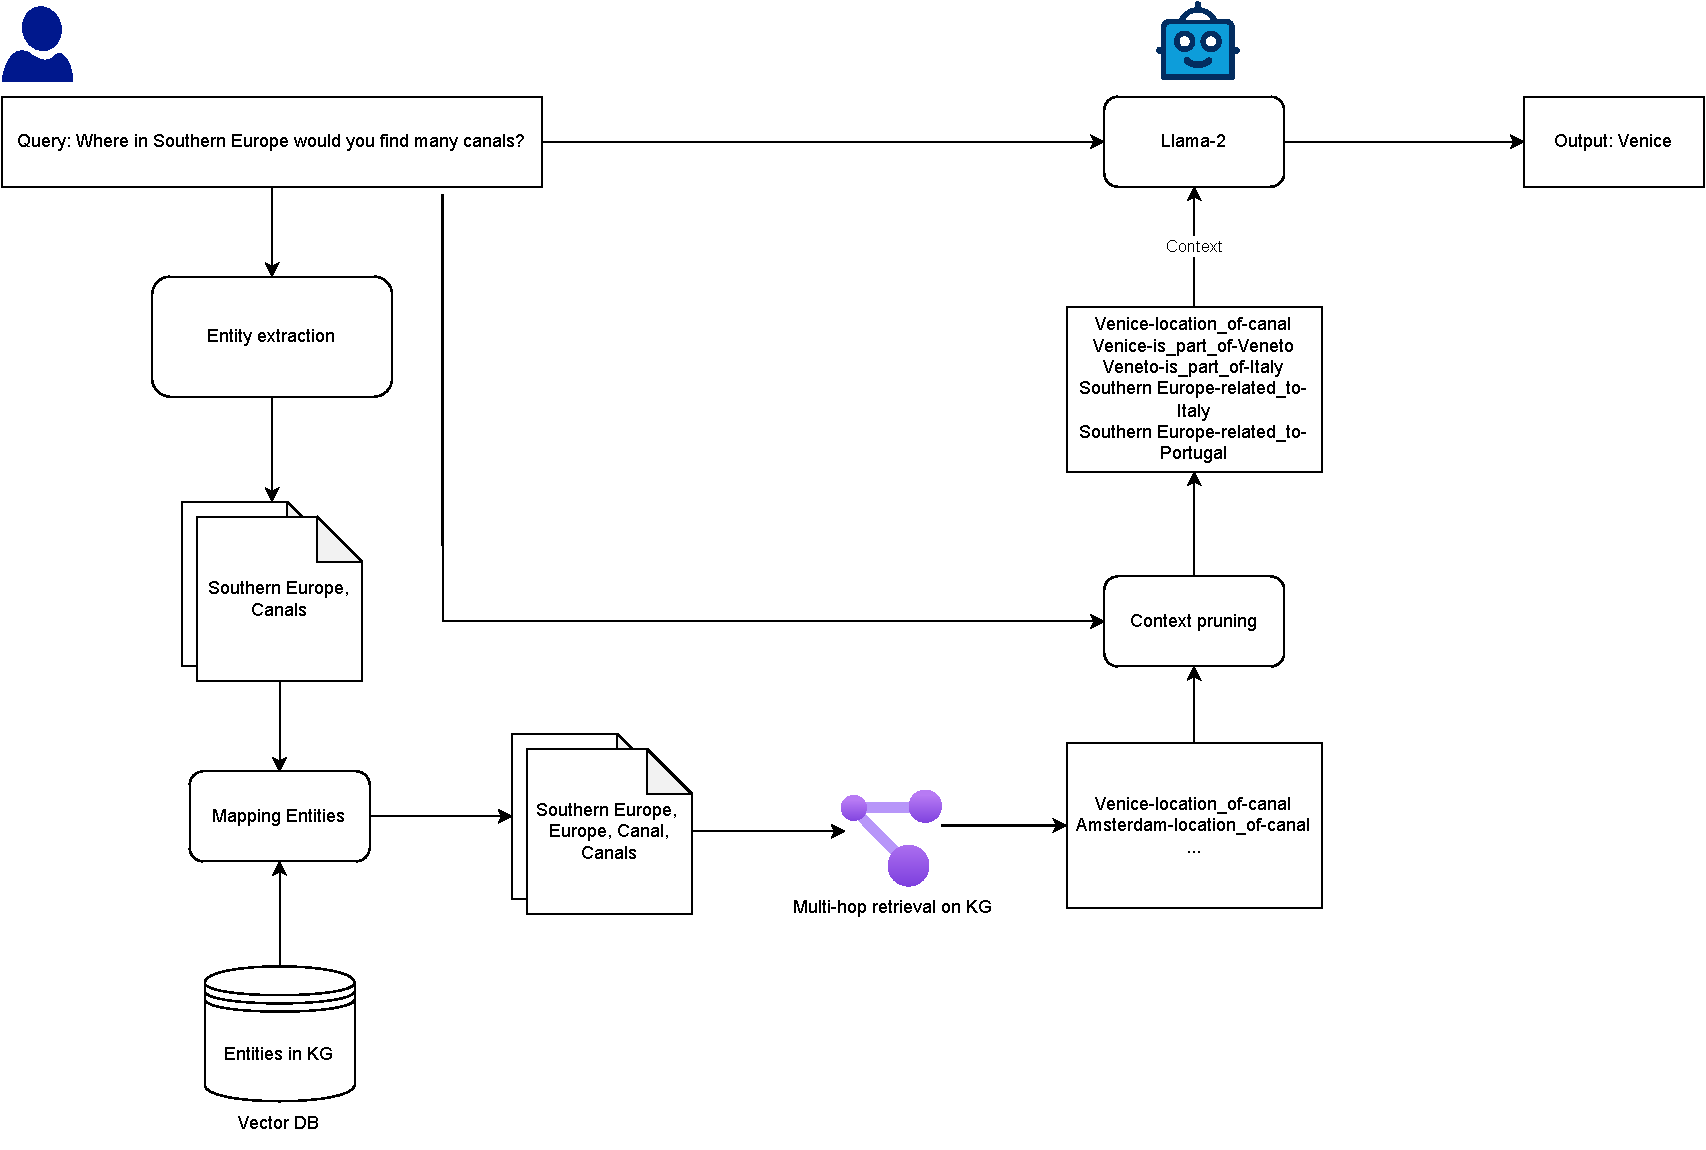
\includegraphics[width=0.95\linewidth]{experiements/image/kg-rag.pdf}
    \caption{Pipeline of Knowledge graph-based retrieval-augmented generation}
    \label{fig:p_kg}
\end{figure}

Figure \ref{fig:p_kg} illustrated the pipeline of Knowledge graph-based retrieval-augmented generation. It consists of \textit{Entity extraction}, \textit{Mapping entities}, \textit{Context pruning}, \textit{Multi-hop retrieval on KG}, \textit{Generator}.

\textbf{Preprocessing data}: Each entity in knowledge graph is projected to latent space by using Bi-encoder in order to construct vector database.

\textbf{Entity extraction}: Named Entity Recognition (NER) is a fascinating task that involves identifying and classifying entities like names of people, organizations, locations, and other important terms within a given text. In this project, Llama-2 is used as an NER tool to detect entities in a sentence. The sample generation can be referred in Appendix \ref{apd:A}.

\textbf{Mapping entities}: In this project, the Bi-encoder is used to map the extracted entities to the same latent space as the entities in the vector database, then compared with each entities' vector by cosine similarity. This phase helps to correct the entity, as in some cases, the extracted entity may not exist in the knowledge graph. Therefore, it can be found a entity which is similar to the extracted entity.
If there are no extracted entities, the user’s query can be used to find relevant entities by mapping the query to the latent space and then comparing it with each entity’s vector.

\textbf{Multihop-retrieval on KG}: The next step is to find the relevant knowledge on the knowledge graph after mapping the entities. This can be done by selecting the top-K neighbor hops for each entity. The extracted knowledge is represented as triplets of the form (<Entity>,<Relation>,<Entity>). Each triplet is then converted into a sentence as shown in Figure \ref{fig:p_kg}.

\textbf{Context pruning}: Cross-encoder is employed to make comparison between query and each triplet, and after that top-K' triplets are extracted based on the similarity score and passed to generator to answer the the query from user.